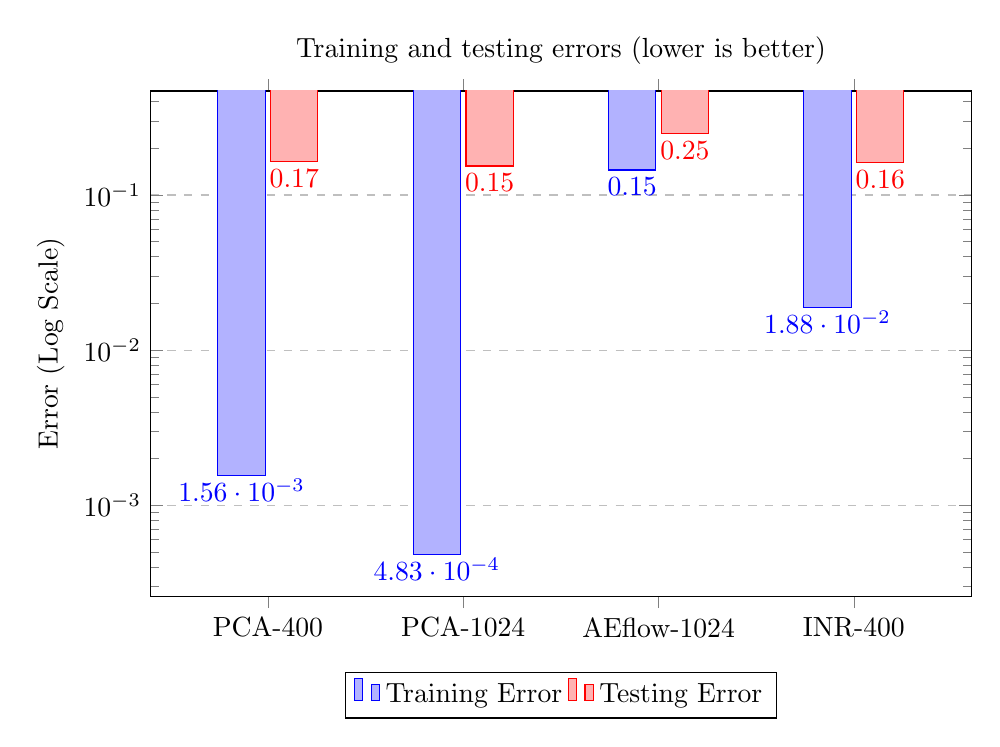
\begin{tikzpicture}
	\begin{axis}[
			title={Training and testing errors (lower is better)},
			ybar,
			ylabel={Error (Log Scale)},
			symbolic x coords={PCA-400, PCA-1024, AEflow-1024, INR-400},
			xtick=data,
			nodes near coords,
			nodes near coords align={vertical},
			every node near coord/.append style={yshift=-3ex},  % Shift the y coordinate labels up
			point meta=rawy,
			width=12cm,
			height=8cm,
			bar width=0.6cm,  % Increase the width of the bars
			enlarge x limits=0.2,
			ymode=log,  % Change Y-axis to log scale
			legend style={at={(0.5,-0.15)},
					anchor=north,legend columns=-1},
			ymajorgrids=true,
			grid style=dashed
		]
		\addplot coordinates {(PCA-400,1.56e-3) (PCA-1024,4.83e-4) (AEflow-1024,0.145) (INR-400,1.88e-2)};
		\addplot coordinates {(PCA-400,0.165) (PCA-1024,0.154) (AEflow-1024,0.251) (INR-400,0.162)};
		\legend{Training Error, Testing Error}
	\end{axis}
\end{tikzpicture}